\section{Performance Graphs}

By using more cores to speedup the program you expect the runtime to be inversely proportional to the number of cpu cores used.

\begin{equation}
\text{runtime} = \frac{\text{runtime with one core}}{\text{\#cores}}
\label{eq:runtime}
\end{equation}

This is true if the whole program can be run in parallel. You can see this general dependency in \autoref{fig:scalingTheory}. For small grid sizes the overhead for managing multiple threads becomes dominating and opposes the speedup - clearly visible in \autoref{fig:scaling}. Another important aspect is memory bandwidth. In modern computer systems the speed of a program is often determined by the speed of memory access. One has to pay attention to this fact also when parallelizing a program. The optimal performance can only be reached when each core has optimal memory access. In our test system we have 4 cpus with dedicated memory and 8 cores each. So our first 4 threads have optimal memory access but the fifth thread has to share memory bandwidth with our first thread. This results in the small kink which is visible in \autoref{fig:scalingTheory}.

\begin{figure}
	\centering
		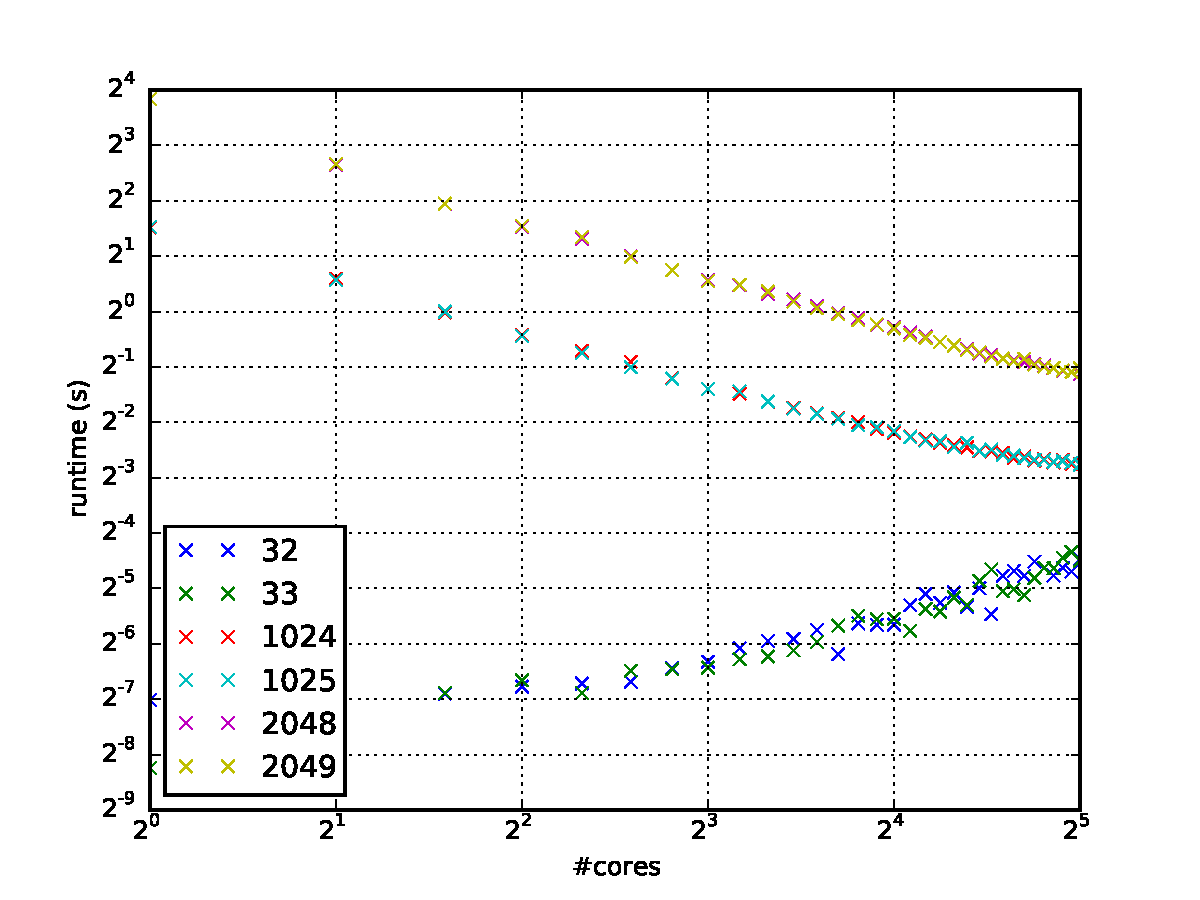
\includegraphics[width=0.80\textwidth]{../img/scaling.pdf}
	\caption{Runtime for different grid sizes with respect to the number of cpu cores used. For small system sizes the management overhead is dominant. The expected behavior can be seen for larger system sizes.}
	\label{fig:scaling}
\end{figure}

\begin{figure}
	\centering
		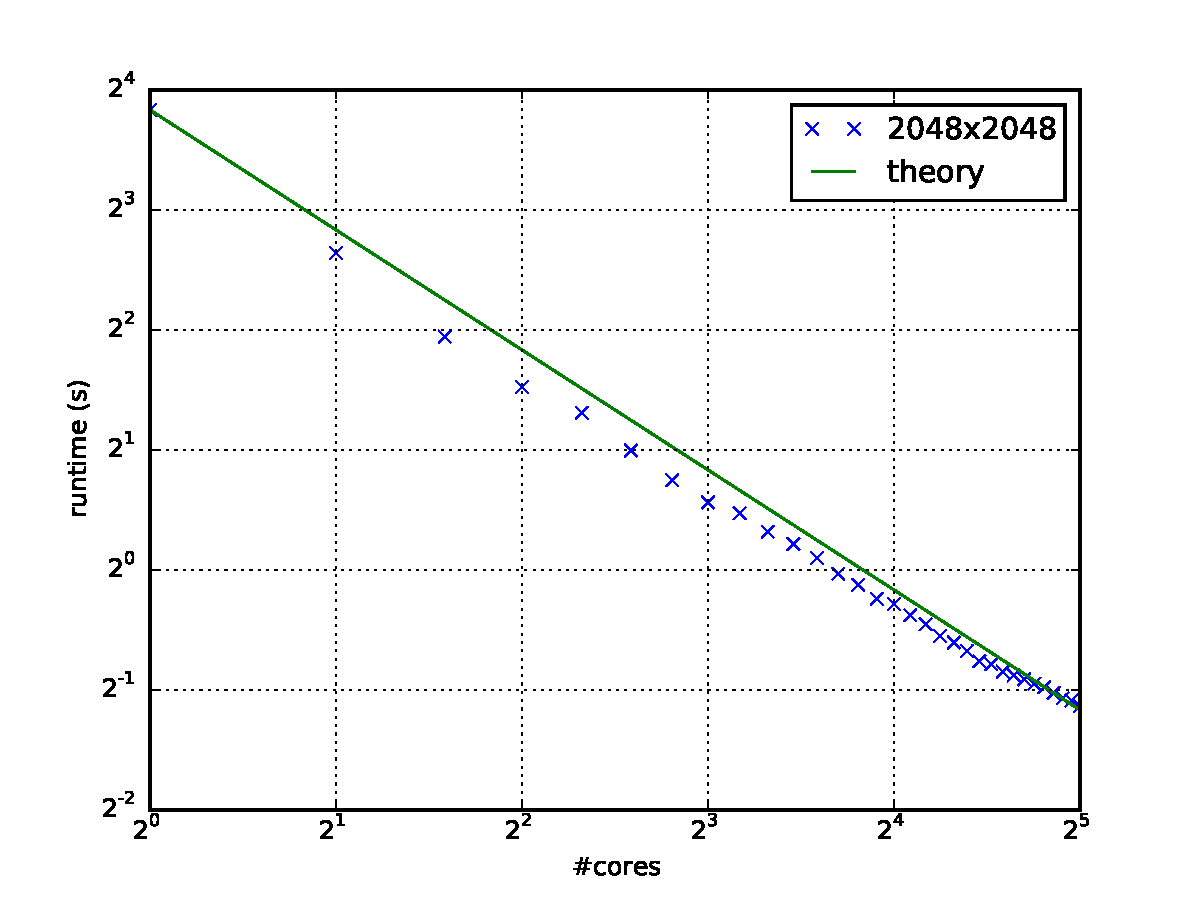
\includegraphics[width=0.80\textwidth]{../img/scalingTheory.pdf}
	\caption{Runtime for a system of size 2048. The theoretically expected runtime according to \autoref{eq:runtime} is also plotted for comparison.}
	\label{fig:scalingTheory}
\end{figure}
